% VUT FIT MITAI
% MSZ 2021/2022
% Author: Vladimir Dusek
% Login: xdusek27

%%%%%%%%%%%%%%%%%%%%%%%%%%%%%%%%%%%%%%%%%%%%%%%%%%%%%%%%%%%%%%%%%%%%%%%%%%%%%%%%

% Path to figures
\graphicspath{{bms/bezdratove_lokalni_site/figures}}

%%%%%%%%%%%%%%%%%%%%%%%%%%%%%%%%%%%%%%%%%%%%%%%%%%%%%%%%%%%%%%%%%%%%%%%%%%%%%%%%

\chapter{BMS -- Bezdrátové lokální sítě (Wifi, Bluetooth).}

% Otazka MSZ 2020, 113 MSK
% [Ocenasek] Bezpecnost bezdratovych siti, chvili me nechal mluvit, tak jsem rekl neco k WEPu, pak uz to bylo stylem otazka odpoved. Zajimala ho proudova sifra WEPu, TKIP ve WPA, WPA enterprise a 802.1x, ale vetsinou chtel vedet spis veci obecneho charakteru, napr. jake jsou vyhody WPA enterprise oproti PSK a tak

%%%%%%%%%%%%%%%%%%%%%%%%%%%%%%%%%%%%%%%%%%%%%%%%%%%%%%%%%%%%%%%%%%%%%%%%%%%%%%%%

\section{Zdroje}

\begin{compactitem}
    \item \path{08-bezdratove_lan.pdf}
    \item \path{BMS_2020-12-02.mp4} % Todo: cas 7:35
    \item \path{BMS_2020-12-09.mp4}
\end{compactitem}

%%%%%%%%%%%%%%%%%%%%%%%%%%%%%%%%%%%%%%%%%%%%%%%%%%%%%%%%%%%%%%%%%%%%%%%%%%%%%%%%

\section{Bezdrátová komunikace}

\begin{compactitem}
    \item Princip bezdrátové komunikace a jednotlivé fáze přenosu.
\end{compactitem}

\begin{compactenum}
    \item \textbf{Kódování hlasu a digitalizace} \begin{compactitem}
        \item Z analogového hlasu uděláme digitální signál.
        \item Velká redundance, provádíme kompresy.
        \item Dojde ke ztrátě nějakých informací a přidání šumu (kvantizační šum) při dekódování.
        \item Např. pulzně kódová modulace (PCM, \textit{pulse-code modulation}).
    \end{compactitem}

    \item \textbf{Kódování kanálu} \begin{compactitem}
        \item Data přenáším přes rádiové kanály (eventualně infračervené záření), které jsou nespolehlivé (data mohu ztratit, bit může přeskočit, \dots).
        \item Počítáme s tím, zavádíme redundanci tak, aby bylo možné většinu chyb opravit. \begin{compactitem}
            \item Chceme minimalizovat opětovné přenášení (to je problém).
            \item Detekce chyb pomocí BER -- Bit Error Rate, FER -- Frame Error Rate.
        \end{compactitem}
        \item Zvyšuje se tím výrazně objem dat.
        \item Metody: \begin{compactitem}
            \item Blokové korekční kódy (Hammingův kód) -- vstup je rámec, výstup je původní rámec + zabezpečovací bity.
            \item Konvoluční korekční kódy -- nezná pojem rámec, vstupují bity a vystupují bity rychleji.
            \item Turbo korekční kódy.
        \end{compactitem}
    \end{compactitem}

    \item \textbf{Prokládání (\textit{interleaving})} \begin{compactitem}
        \item Pokud se na kanálu objevuje nějaké rušení, tak je většinou impulsní a zaruší se několik bitů vedle sebe.
        \item To se nelíbí mechanismům kódování kanálu, ty mají rády pokud je zarušen \uv{sem tam} nějaký bit, ale ne shluk vedle sebe.
        \item Zabraňujeme tomu tak, že prohazujeme pořadí jednotlivých bitů.
    \end{compactitem}

    \item \textbf{Šifrování dat} \begin{compactitem}
        \item Může být v různé fázi, není shoda.
        \item Umístění šifrování tak jak ve schématu je problém, jelikož se mohou objevit chyby díky přenosu, což se většine šifrovacích algoritmů nelíbí, proto by dávalo smysl to umístit až za (de)kódování kanálu.
    \end{compactitem}

    \item \textbf{Modulace} \begin{compactitem}
        \item Dostat náš signál do analogové podoby pro přenos a na potřebnou frekvenci (úprava frekvencí, amplitud, fází).
        \item Také prováděn multiplexing (přenášení více signálů přes jednu anténu).
    \end{compactitem}

    \item \textbf{Přenos signálu přes telekomunikační síť} \begin{compactitem}
        \item Jak bylo řečeno výše, jde o nespolehlivý přenos přes rádiové (nebo historicky infračervené) záření.
    \end{compactitem}

    \item \textbf{Demodulace} \begin{compactitem}
        \item Dostat signál z podoby vhodné pro přenos na podobu vhodnou pro dekódování (úprava frekvencí, amplitud, fází).
        \item Prováděn demultiplexing.
    \end{compactitem}

    \item \textbf{Dešifrování} \begin{compactitem}
        \item Dešifrování, platí to stejné jako u šifrování.
    \end{compactitem}

    \item \textbf{Prokládání (\textit{deinterleaving})} \begin{compactitem}
        \item Překládání bitů analogicky k prokládání na druhé straně.
    \end{compactitem}

    \item \textbf{Dekódování kanálu} \begin{compactitem}
        \item Opravení chyb.
    \end{compactitem}

    \item \textbf{Dekódování hlasu} \begin{compactitem}
        \item Pokud chceme řeč, tak převod do analogové podoby.
    \end{compactitem}
\end{compactenum}

\begin{figure}[H]
    \centering
    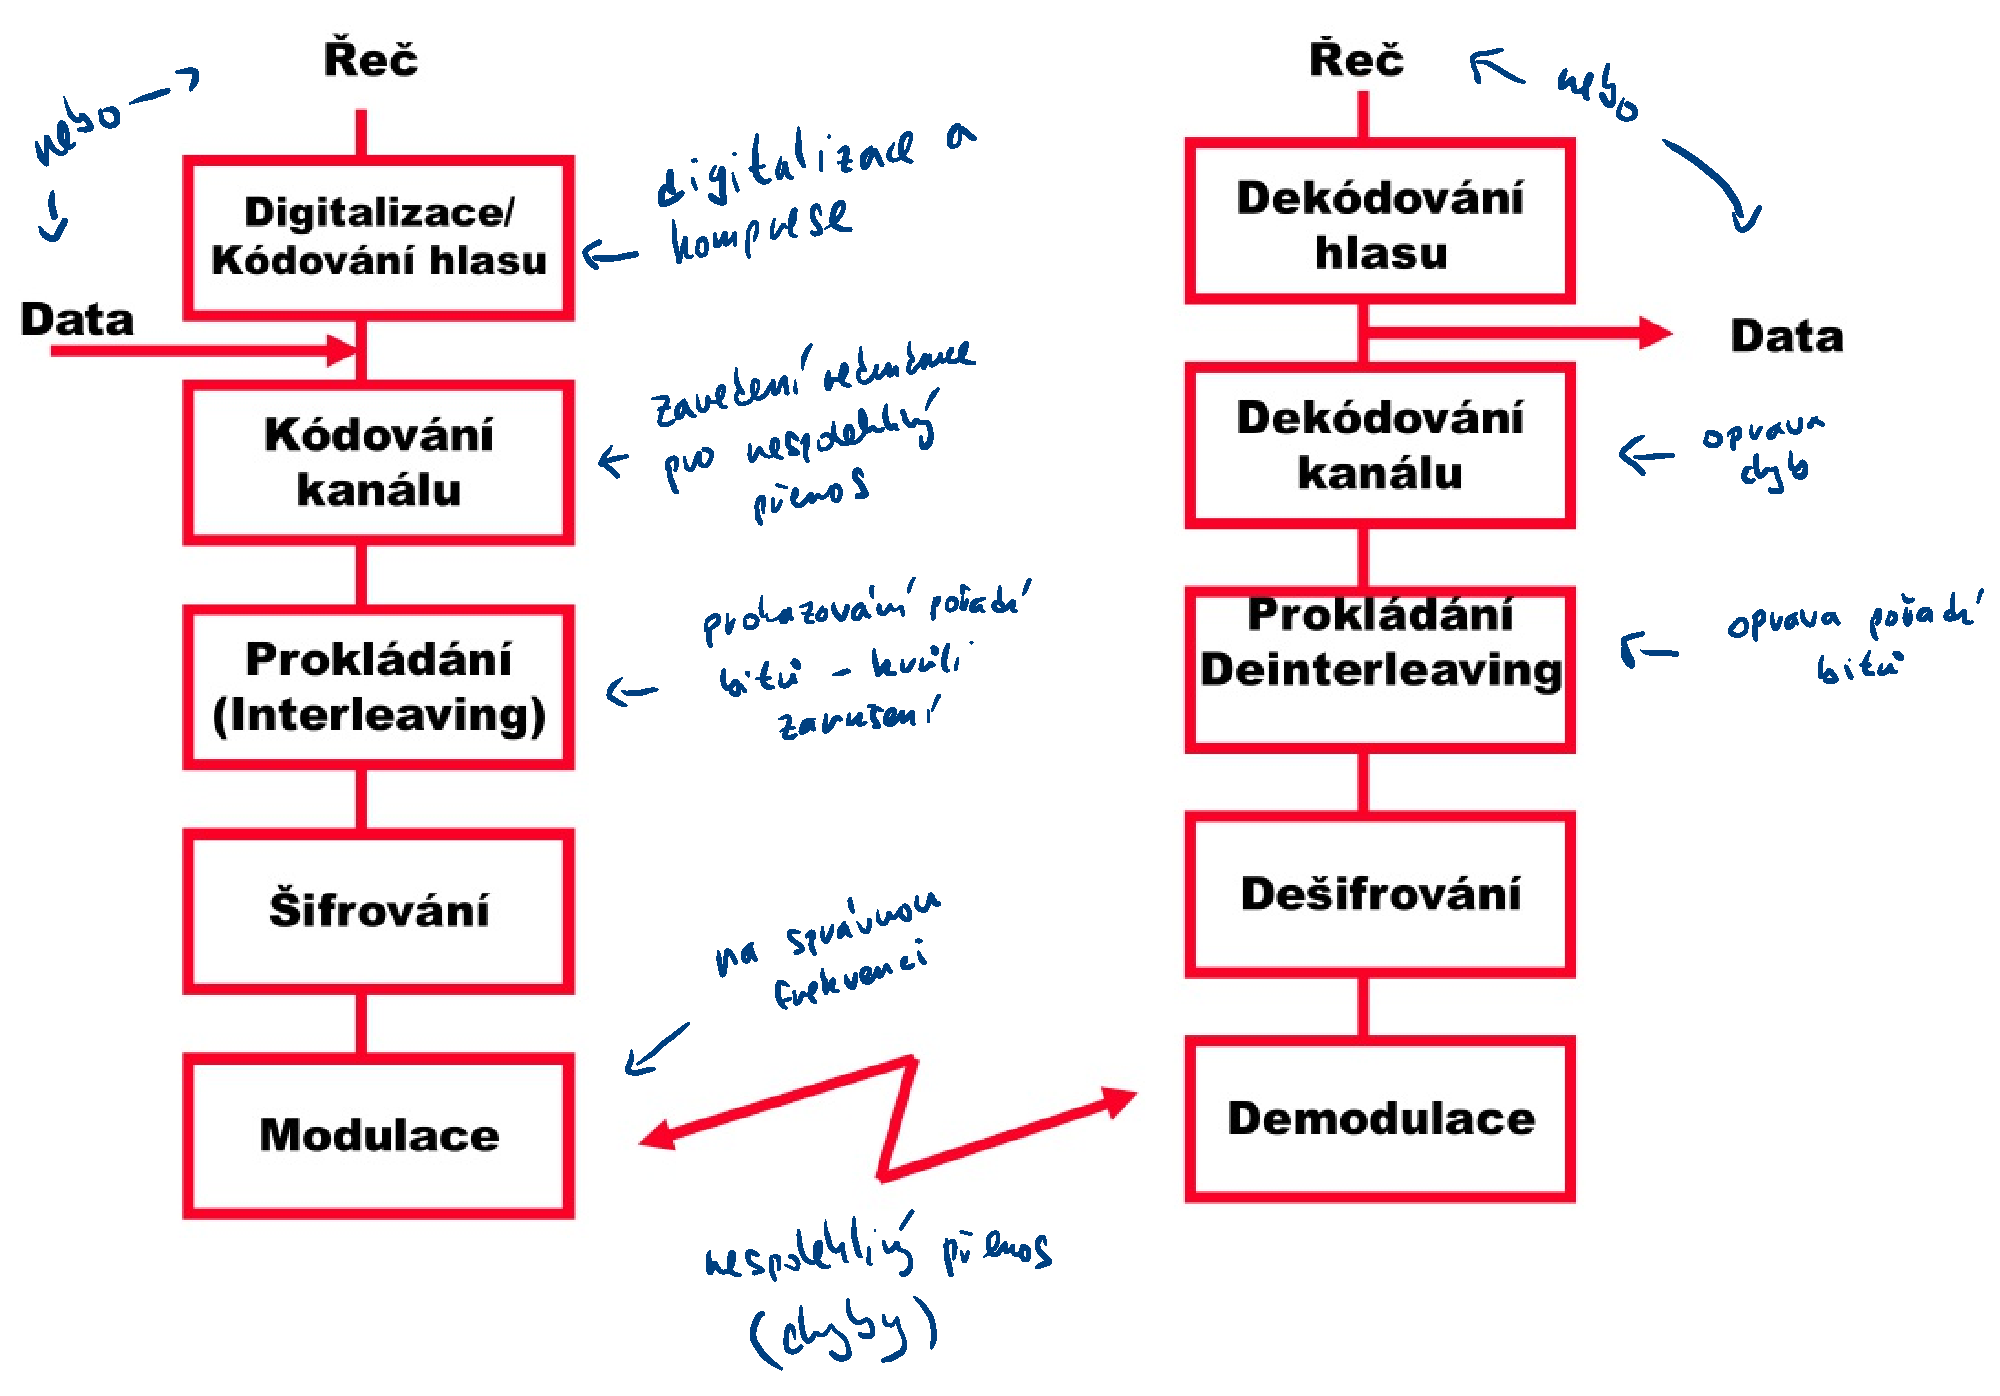
\includegraphics[width=1\linewidth]{bezdratova_komunikace.pdf}
    \caption{Schéma bezdrátové komunikace.}
\end{figure}

%%%%%%%%%%%%%%%%%%%%%%%%%%%%%%%%%%%%%%%%%%%%%%%%%%%%%%%%%%%%%%%%%%%%%%%%%%%%%%%%

\section{Modulace}

\todo{todo}

%%%%%%%%%%%%%%%%%%%%%%%%%%%%%%%%%%%%%%%%%%%%%%%%%%%%%%%%%%%%%%%%%%%%%%%%%%%%%%%%

\section{Sdílení spektra}

\begin{compactitem}
    \item Metoda přístupu ke kanálu (\textit{channel access method}) umožňuje více než dvěma koncovým zařízením připojeným ke stejnému přenosovému médiu přenášet přes něj a sdílet jeho kapacitu (a to tak, aby se vzájemně nerušili).

    \item Metoda přístupu ke kanálu je založena na sdílení spektra (multiplexing), které umožňuje několika datovým tokům nebo signálům sdílet stejný komunikační kanál nebo přenosové médium. V této souvislosti multiplexování zajišťuje fyzická vrstva.

    \item Mnoho přístupů: \begin{compactenum}
        \item \textbf{Prostorový multiplex} (SDMA, \textit{space-division multiple access}) \begin{compactitem}
            \item Jsme schopni využít 1 frekvenci pro více účastníků, jsou-li fyzicky daleko od sebe.

            \item Je potřeba ochranný interval.
        \end{compactitem}

        \item \textbf{Frekvenční multiplex} (FDMA, \textit{frequency-division multiple access}) \begin{compactitem}
            \item Rozdělení spektra na menší úseky (kanály), které poté přidělujeme účastníkům.
            \item Kanál má 2 atrbitu: šířku a střední frekvenci.
            \item Nevýhoda: plýtvání pásmem, nutnost ochranných intervalů.
        \end{compactitem}

        \item \textbf{Časový multiplex} (TDMA, \textit{time-division multiple access}) \begin{compactitem}
            \item Kanál dostane celé spektrum po určitý čas.
            \item Nelze použít v analogovém vysílání.
            \item Nutná synchronizace.
            \item Jedna nosná, vysoká propustnost.
        \end{compactitem}

        \item \textbf{Časový a frekvenční multiplex} (FTDMA, \textit{frequency and time division multiple access}) \begin{compactitem}
            \item Kombinace časového a frekvenčního multiplexingu.
            \item Každý účastník dostane kanál a časový slot (kde a kdy komunikuje).
            \item Využívá se v GSM.
            \item Nutná časová i frekvenční koordinace.
        \end{compactitem}

        \item \textbf{Kódový multiplex} (CDMA) -- viz dále.

        \item \textbf{Ortogonální multiplex s frekvenčním dělením} (OFDM)-- viz dále.
    \end{compactenum}
\end{compactitem}

\subsection{Kódový multiplex (CDMA)}

\begin{compactitem}
    \item Všichni vysílají na jednom kanálu po celou dobu. \begin{compactitem}
        \item  Nesnažíme se bránit vzájemnému zarušení, to bereme jak osoučást systému.
    \end{compactitem}

    \item Všichni dostávají signál všech a musí si extrahovat informace pro sebe. \begin{compactitem}
        \item signál všech $\rightarrow$ algoritmus $\rightarrow$ signál účastníka

        \item Každá stanice má své unikátní číslo, pokud přijímač toto číslo zná, může se \uv{naladit} (z čísla derivujeme \uv{náhodný} signál).
    \end{compactitem}

    \item Nevýhoda: složitost přijímače (potřeba počítač pro kódování / dekódování).

    \item Výhoda: žádné ochranné intervaly, žádná koordinace a synchronizace, odolnost proti rušení, ochrana proti odposlouchávání.
\end{compactitem}

\begin{figure}[H]
    \centering
    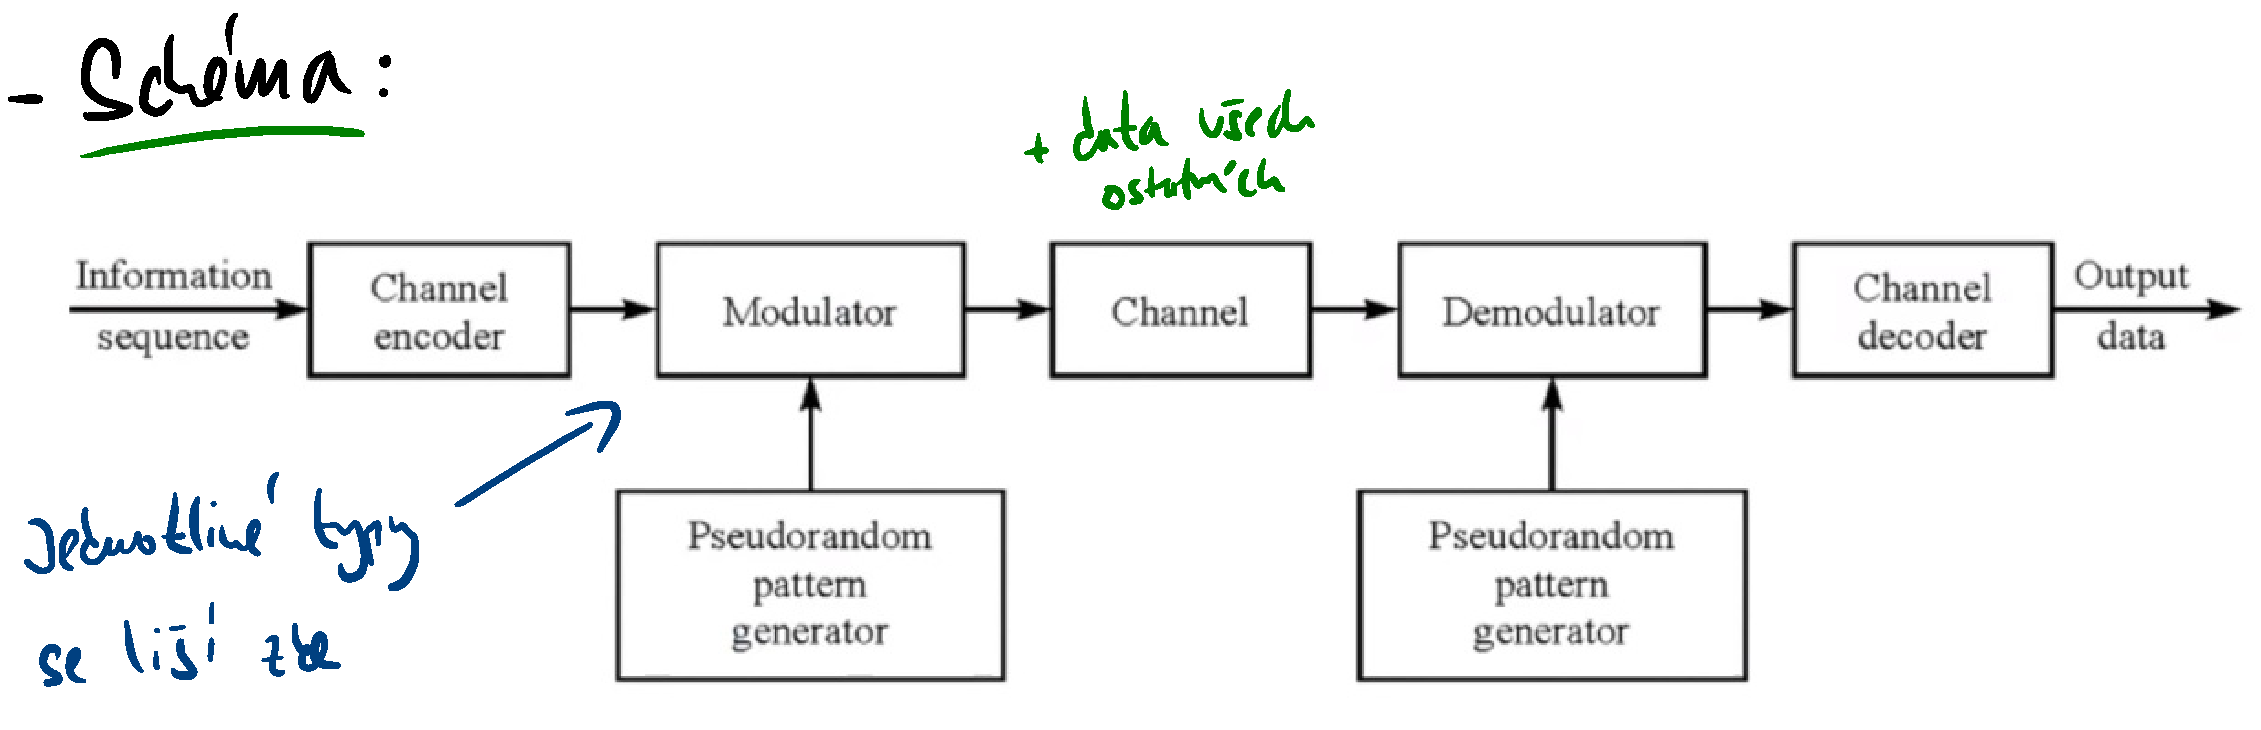
\includegraphics[width=1\linewidth]{cdma.pdf}
    \caption{CDMA schéma.}
\end{figure}

\subsubsection{DSSS (\textit{direct sequence spread spectrum})}

\begin{compactitem}
    \item \uv{Rozprostřené spektrum}.
    \item Užitečný signál $\oplus$ (XOR) vygenerovaný náhodný signál.
    \item Výsledek se namoduluje a posílá.
\end{compactitem}

\begin{figure}[H]
    \centering
    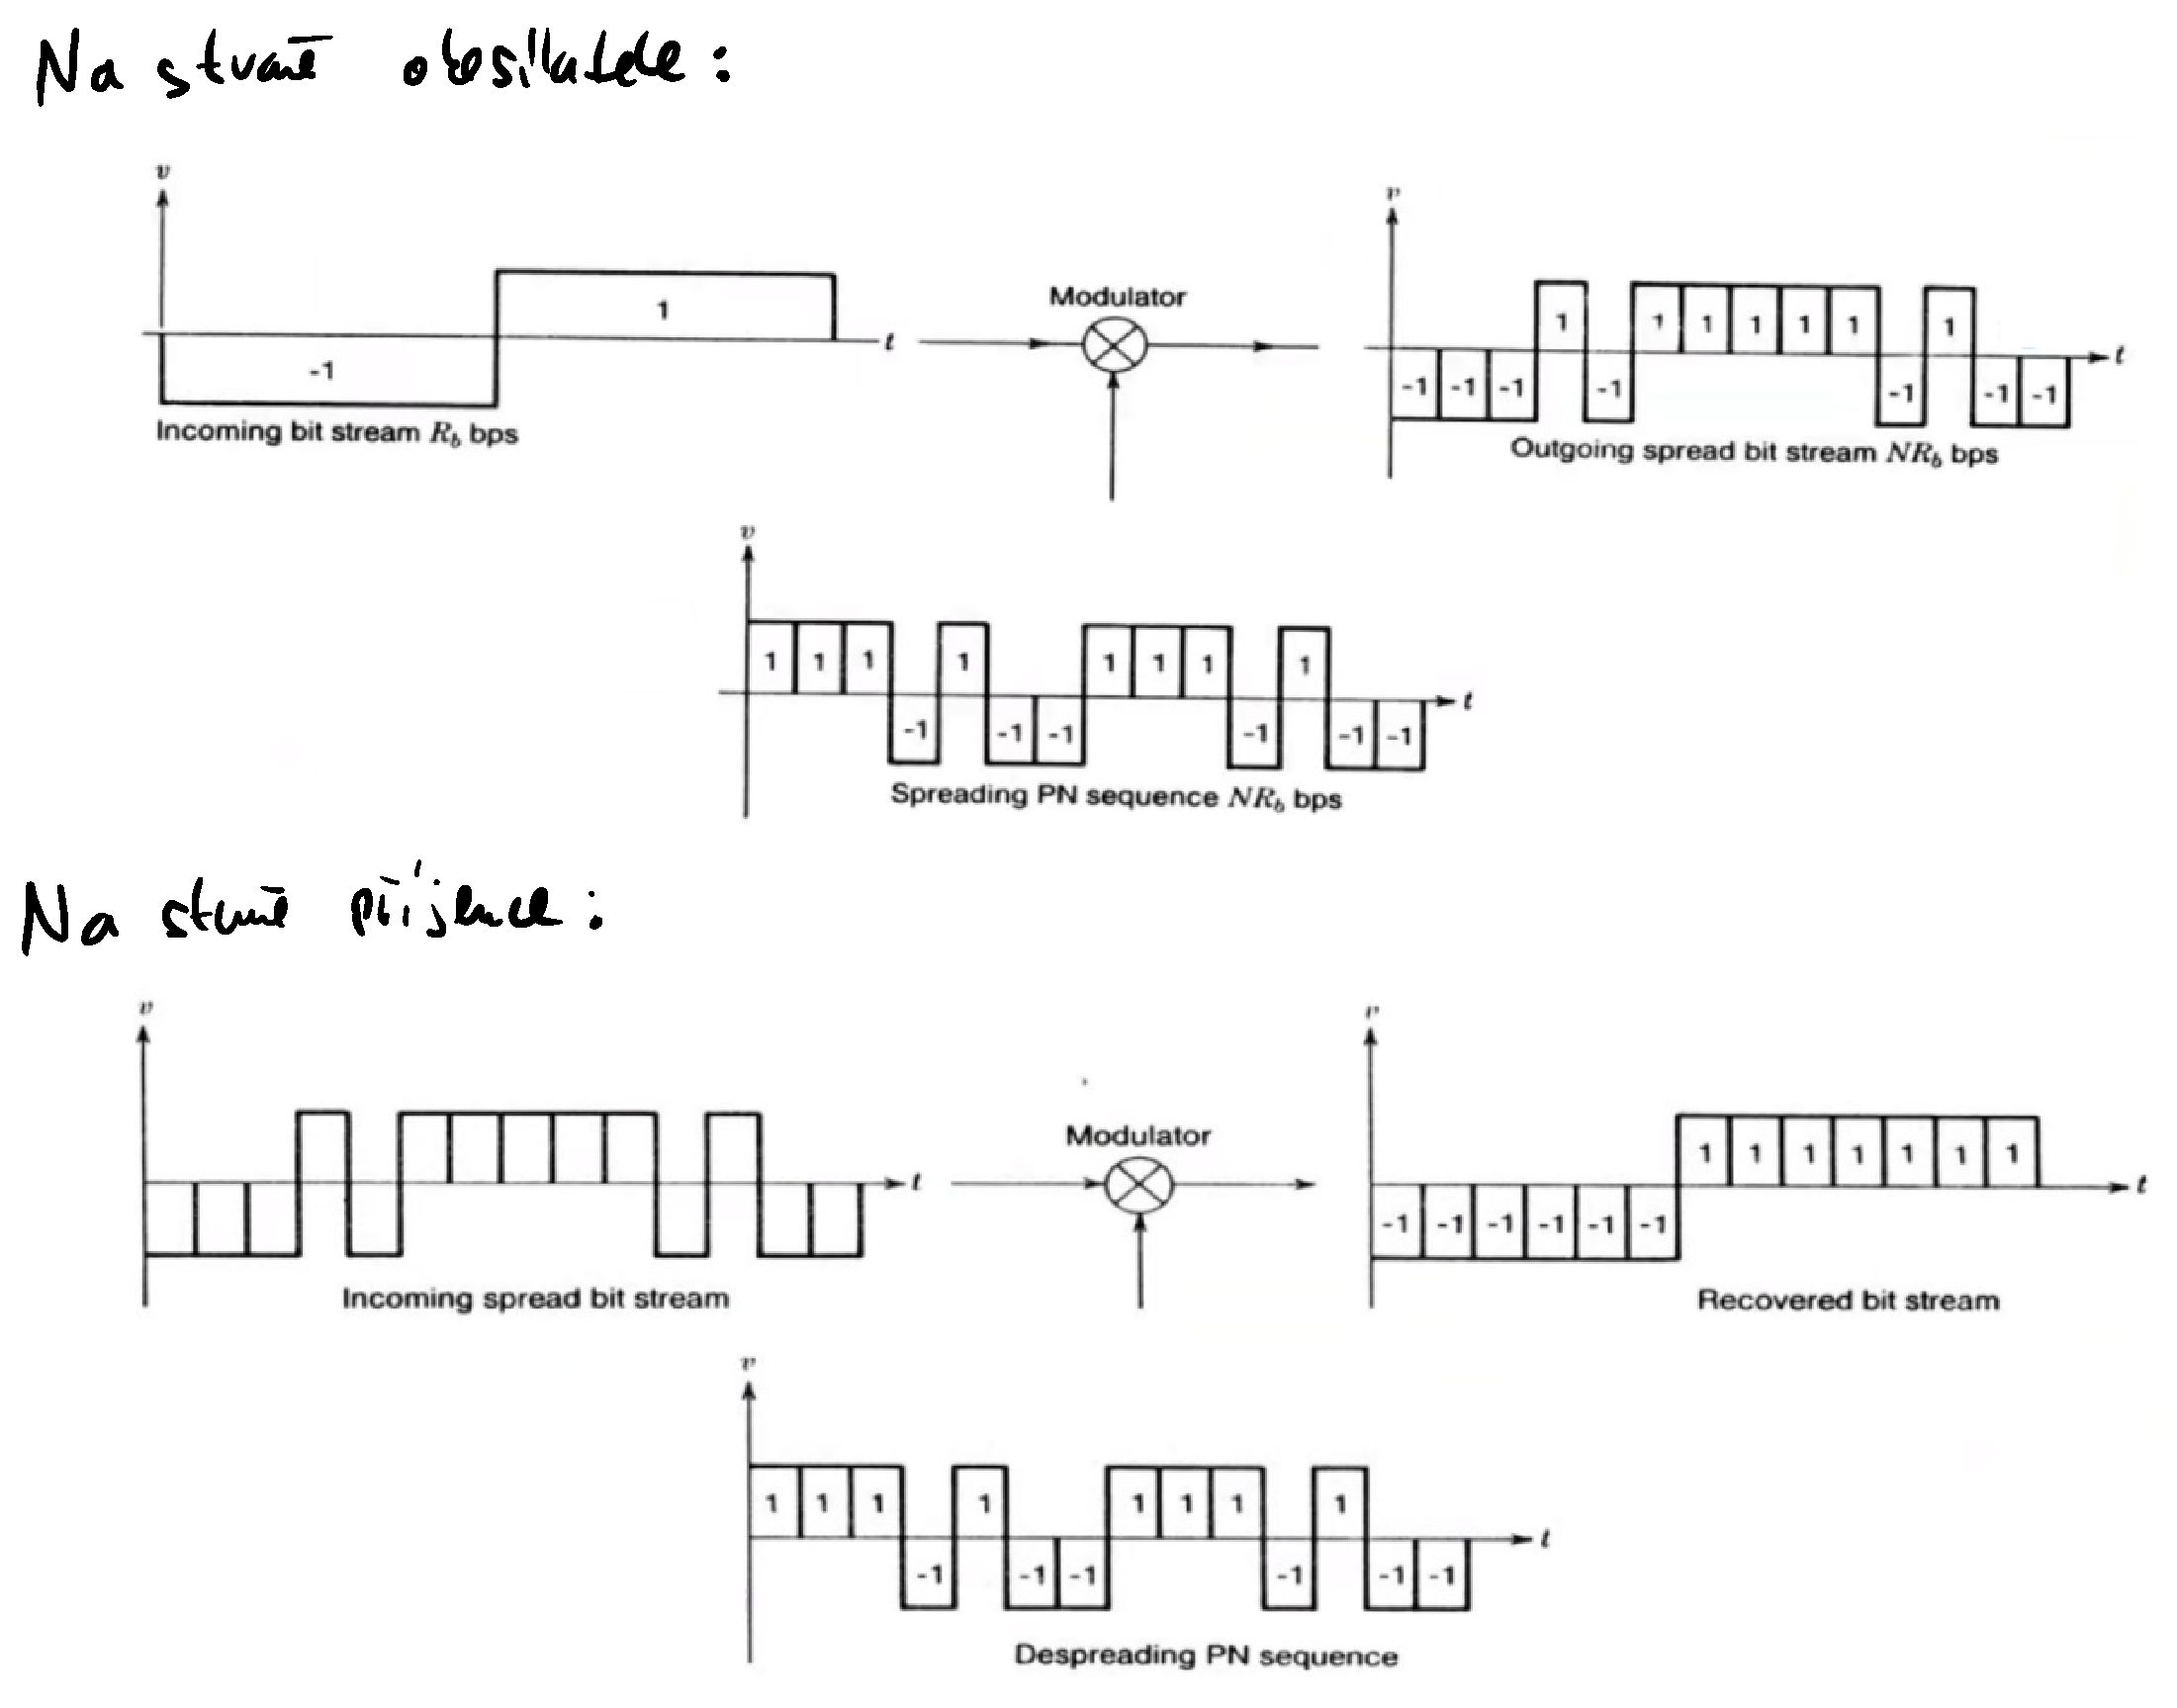
\includegraphics[width=1\linewidth]{dsss.pdf}
    \caption{DSSS.}
\end{figure}

\subsection{Ortogonální multiplex s frekvenčním dělením (OFDM)}

\begin{compactitem}
    \item Ortogonální multiplex s frekvenčním dělením (OFDM, \textit{orthogonal frequency division multiplexing})

    \item Přenos je rozložen do mnoha úzkých subkanálů, které jsou přenášeny paralelně.

    \item Umožňuje, aby se postranní pásma subkanálů překrývala, což šetří pásmo.

    \item Přijímač je schopen oddělit překrývající se subkanály, protože jsou ortogonální.
\end{compactitem}

\todo{todo}

%%%%%%%%%%%%%%%%%%%%%%%%%%%%%%%%%%%%%%%%%%%%%%%%%%%%%%%%%%%%%%%%%%%%%%%%%%%%%%%%

\section{Bezdrátové lokální sítě}

\begin{compactitem}
    \item \textbf{Výhody} \begin{compactitem}
        \item Velmi flexibilní -- nemusíme natahovat dráty.
        \item Možnost ad-hoc sítí bez předchozího plánování.
        \item Téměř žádné problémy s vedením (historické budovy, požární přepážky).
        \item Robustnější vůči nehodám (nehrozí přerušení vodičů).
    \end{compactitem}

    \item \textbf{Nevýhody} \begin{compactitem}
        \item Nižší přenosová rychlost oproti drátovým sítím (1-10 Mbit/s). \begin{compactitem}
            \item Máme pouze omezené frekvence, na kterých můžeme přenášet data.
        \end{compactitem}
        \item Mnoho proprietárních řešení, standardizace trvá nějakou dobu (např. IEEE 802.11).
        \item Produkty musí dodržovat mnoho různých omezení pro bezdrátové přístroje (frekvenční plánování, výkony, homologace, \dots), vytvořit globální řešení trvá delší dobu.
    \end{compactitem}

    \item \textbf{Cíle návrhu} \begin{compactitem}
        \item Globální provoz. \begin{compactitem}
            \item Historicky problémy vzhledem k různým legislativám ohledně rádiového vysílání v jednotlivých státech.
        \end{compactitem}
        \item Nízká spotřeba pro provoz z baterií.
        \item Bezpečnost -- Bezdrátové sítě se snáze odposlouchávají, než drátové, proto je šifrování nutnost.
        \item Transparentnost k vyšším protokolům. \begin{compactitem}
            \item Např. TCP/IP neví jestli běží po drátové/bezdrátové technologii.
        \end{compactitem}
    \end{compactitem}

    \item Jako fyzické médium se používá \textbf{rádiový přenos} (typicky bezlicenční pásmo 2,4\,GHz), ačkoliv historicky byl ve hře i infračervený přenos.

    \item \textbf{Infrastrukturní síť} -- Máme nějakou infrastrukturu (\textit{access point}), ke které se připojují klienti.

    \item \textbf{Adhoc sítě} -- Náhodně se potká několik bezdrátových zařízení a propojí se.
\end{compactitem}

%%%%%%%%%%%%%%%%%%%%%%%%%%%%%%%%%%%%%%%%%%%%%%%%%%%%%%%%%%%%%%%%%%%%%%%%%%%%%%%%

\section{WiFi}

\begin{compactitem}
    \item WiFi (\textit{wireless local area network}), několik verzí standardu IEEE 802.11.

    \item Specifikuje fyzickou vrstvu ($L_0$) a vrstvu síťového rozhraní ($L_1$) v TCP/IP stacku, resp. ISO/OSI.

    \item Fyzická vrstva -- fyzické médium (rádiové, infračervené vysílání) + vrstva konvergence, která zapouzdřuje médium.

    \item Vrstva síťového rozhraní (vrstva přístup k médiu) -- přístup k médiu, fragmentace, šifrování, detekce a korekce chyb. \begin{compactitem}
        \item Zajišťuje přístup k fyzickému médie
    \end{compactitem}
\end{compactitem}

\begin{figure}[H]
    \centering
    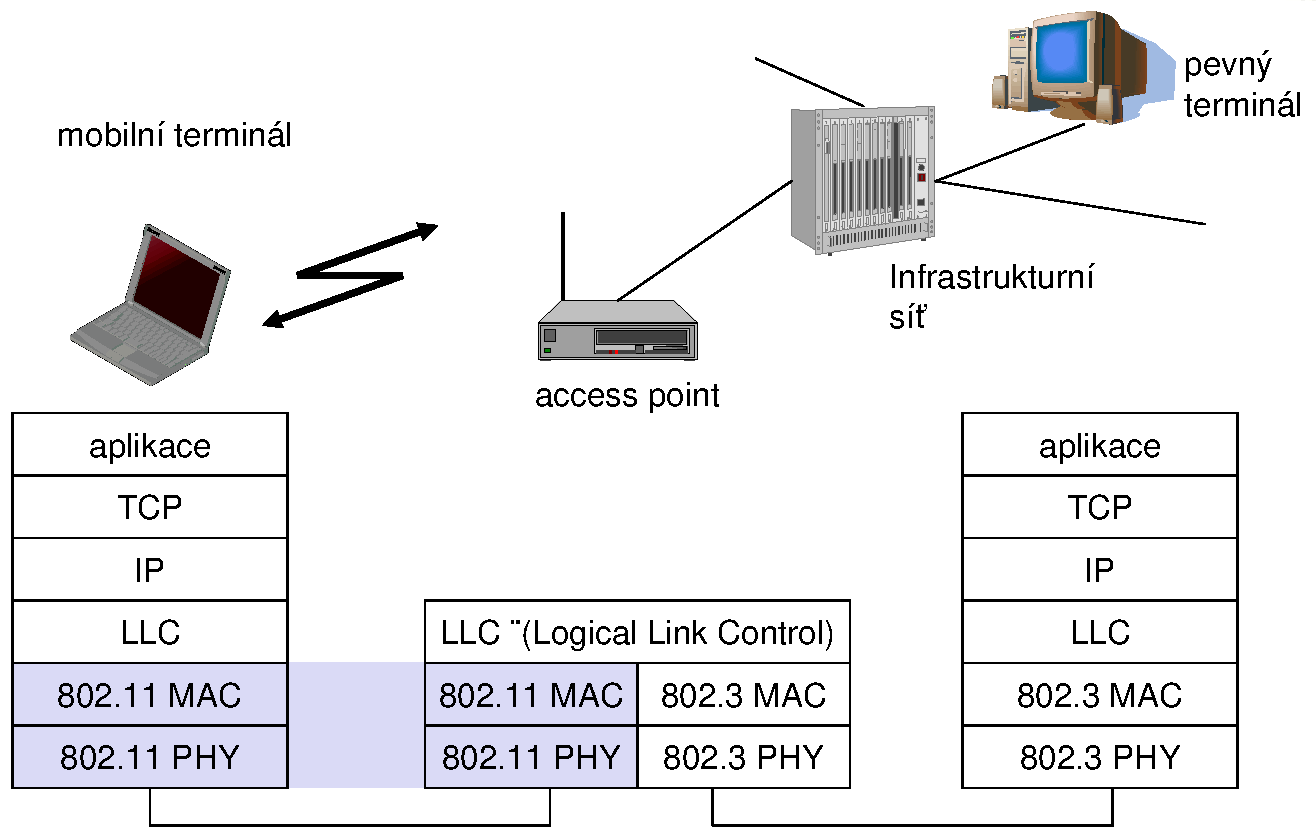
\includegraphics[width=0.75\linewidth]{wifi-architektura.pdf}
    \caption{IEEE 802.11 WiFi architektura.}
\end{figure}

\subsection{IEEE 802.11}

\begin{compactitem}
    \item Pásmo: 2,4\,GHz.

    \item Maximální rychlost: 2\,Mbitps.

    \item Fyzická vrstva: \begin{compactitem}
        \item rádiové kanály, multimplexing CDMA (\textit{code division multiple access}), konkrétně DSSS (\textit{direct sequence spread spectrum}),
        \item rádiové kanály, CDMA, konkrétně FHSS, zahynulo.
        \item infračervené kanály, zahynulo.
    \end{compactitem}

    \item Fyzická vrstva, která přežila, má 11 kanálů o šířce 22 MHz, které se překrývají (netypické).
\end{compactitem}

\subsection{IEEE 802.11a}

\begin{compactitem}
    \item Frekvenční pásmo: 5,0\,GHz (přidávají nové ).
    \item Maximální rychlost: 54\,Mbitps
    \item Maximální dosah: 100\,m mimo budovy, 10\,m v budově.
    \item Americká varianta (pouze USA) po 802.11.

    \item Cíl: \begin{compactitem}
        \item přidělení nového frekvenčního pásma, které není tak vytížené (zpětná kompatibilita není nutná),
        \item dosáhnutí vyšší rychlosti,
        \item odstranění infračervených a rádiových FHSS kanálů.
    \end{compactitem}

    \item Jak dosahuje zrychlení? \begin{compactitem}
        \item Díky tomu, že není zpětně kompatibilní, může používat nové sdílení spektra OFDM.
    \end{compactitem}

    \item Modulace: BPSK, QPSK, 16 QAM, 64 QAM.

    \item Zhodnocení: \begin{compactitem}
        \item není zpětně kompatibilní,
        \item je rychlé,
        \item má menší dosah (kvůli vyšší frekvenci, která má vyšší útlum).
    \end{compactitem}
\end{compactitem}

\subsection{IEEE 802.11b}

\begin{compactitem}
    \item Frekvenční pásmo: 2,4\,GHz.
    \item Maximální rychlost: 11\,Mbitps.
    \item Maximální dosah: 300\,m mimo budovy, 30\,m v budově.
    \item Evropská varianta (celosvětové) po 802.11.

    \item Cíl: \begin{compactitem}
        \item původní frekvenční pásmo,
        \item dosáhnutí vyšší rychlosti,
        \item odstranění infračervené a rádiové FHSS fyzické vrstvy,
        \item zpětná kompatibilita (ale pouze 1 fyzická vrstva).
    \end{compactitem}

    \item Sdílení spektra DSSS (rozprostírací sekvence je tzv. Barkerův kód).

    \item Jak dosahuje zrychlení? \begin{compactitem}
        \item Původní modulační schémata DBPSK, DQPSK pro rychlost 2\,Mbitps.
        \item Nové modulační schéma CCK pro 11\,Mbitps.
    \end{compactitem}

    \item Zhodnocení: \begin{compactitem}
        \item je zpětně kompatibilní,
        \item není tak rychlé jako 802.11a,
        \item ale má větší dosah než 802.11a.
    \end{compactitem}
\end{compactitem}

\subsection{IEEE 802.11g}

\begin{compactitem}
    \item Frekvenční pásmo: 2,4\,GHz.
    \item Maximální rychlost: 54\,Mbitps
    \item Rychlé a má velký dosah.

    \item Cíl: \begin{compactitem}
        \item všechno dobré z 802.11a importovat do 802.11b, tj. zachovat frekvenci 2,4\,GHz,
        \item sdílení spektra OFDM,
        \item zpětná kompatibilita s 802.11b.
    \end{compactitem}

\end{compactitem}

\begin{figure}[H]
    \centering
    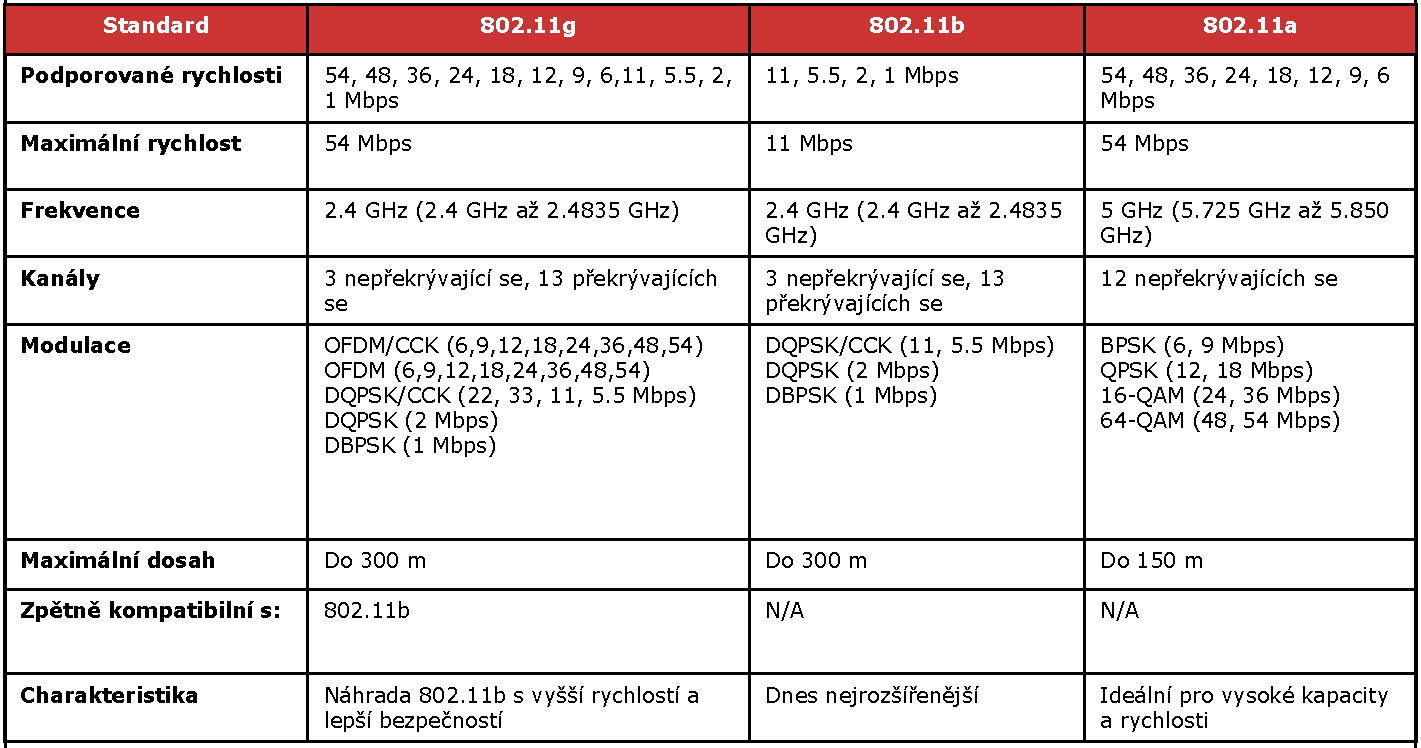
\includegraphics[width=1\linewidth]{802_11_abg.pdf}
    \caption{Srovnání standardů IEEE 802.11 a, b a g.}
\end{figure}

%%%%%%%%%%%%%%%%%%%%%%%%%%%%%%%%%%%%%%%%%%%%%%%%%%%%%%%%%%%%%%%%%%%%%%%%%%%%%%%%

\section{Bluetooth}

Standardizace IEEE.

Wireless Personal Area Network

\todo{todo}


% Popište fyzickou (rádiové vlastnosti a modulaci) a linkovou (topologie) vrstvu Bluetooth stacku. (6 bodů)

% bluetooth, NMT,fm rádio a ještě nějaký, seřadit podle frekvence


% Zacal jsem neco vykladat o frekvencich na jakych bezi wifi a bluetooth. Ze patri do bezlicencnich pasem. Ze patri do VHF a SHF pasem. Pak se me zeptal jak bych v kratkosti charakterizoval wifi a bluetooth. Na to jsem rekl neco o rychlostech, bezpecnosti, spotrebe. Pak jsem zminil standard 802.11. Zminil jsem 2 radiove a jeden infracerveny. Pak jsem uvedl jako priklad 802.11a, rek frekvenci rychlost. Mel jsem pocit, ze povidam tak 2 minuty a p. Skorpil rekl ze mu to staci. EM se na to moc dobre netvaril ale stahnul minutku na nulu a byl konec.

% jaké frekvenční pásmo je používané v standardu 802.15.1


% Ked som si precital tuto otazku tak som si celu tu minutu na vydych hovoril v duchu (FUUUUUUUUUUUU). Zo sieti som poriadne vedel GSM a GPS a vobec som nemal sajny co sa moze spytat z tohto. Tak som zacal ze je to definovane v IEEE 802.11, pod tym existuje viacero verzii, medzi hlavne patria a,b,g. a je pomaly a ma velky dosah, b rychle, maly dosah a g rychle a ma velky dosah. Nasledovala otazka ci viem aky je rozdiel medzi infrastrukturnym a adhoc systemom, tak som vydedukoval ze adhoc vytvorime siet na mieste, infrastrukturny pouzijeme nieco co uz tam je. Prikyvol, tak to bolo snad dobre. Potom este otazka ze aku linkovu vrstvu pouziva wifi, nevedel som. Tak som mal povedat akukolvek. Mal som taky vypadok, ze ani to som nevedel som tresol MAC. To zrusil, ze Ethernet. Tak som mal povedat co je nad tym, som povedal IP. A nakoniec ako funguje NAT (to ani neviem ci je niekde v okruhu, ale som si pamatal z inych predmetov). Takze som dokopy toho moc nepovedal, ani som toho moc nevedel, ale vychadzal som s tym, ze F to nebude urcite.


% Srovnejte Wifi a Bluetooth z hlediska frekvence, dosahu a využití. Popište hlavní výhody a nevýhody Wifi oproti LAN. Popište stručně základní architekturu Wifi. V čem se liší standard 802.11b od základního 802.11? Jak dosahuje vyšší rychlosti? V čem je nevýhoda 802.11a oproti b? Vysvětlete OFDM modulaci. Které verze 802.11 ji využívají? Popište pojmy Pikonet a Scatternet. Co je service discovery protokol?
